\documentclass{math}

\usepackage{enumerate}
\usepackage{graphicx}

\geometry{letterpaper, margin=0.5in}

\title{Boundary Value Problems: Homework 4}
\author{Alvin Lin}
\date{August 2018 - December 2018}

\begin{document}

\maketitle

\subsection*{Problem 1}
Exercises 3.1: problems 1, 2

\subsubsection*{Exercise 1}
Graph the function
\[ f(x) = \begin{cases}
  x &, x<0 \\
  1 &, x=0 \\
  x^2 &, x>0
\end{cases} \]
Determine whether the function is PWC, continuous, PWS, and smooth.
\begin{center}
  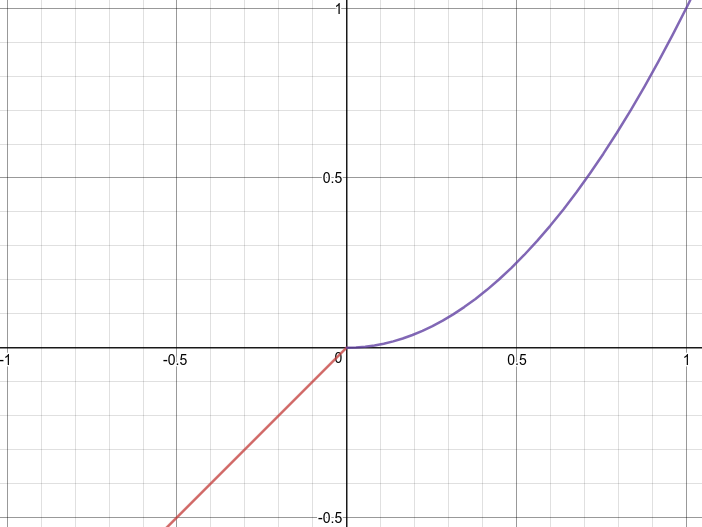
\includegraphics[width=12cm]{assets/hw_04_graph.png}
\end{center}
This function is piecewise continuous and piecewise smooth.

\subsubsection*{Exercise 2}
If \( f(x) = |x| \), is \( f(x) \) continuous at \( x = 0 \)?
\[ \lim_{x\to0_+}f(x) = \lim_{x\to0_-}f(x) = \lim_{x\to0}f(x) = 0 \]
\( f(x) \) is continuous at 0.
\begin{align*}
  f'(0_+) &= 1 \\
  f'(0_-) &= -1
\end{align*}
\( f(x) \) is not differentiable at 0 because the left and right hand
derivatives differ on both sides.

\subsection*{Problem 2}
Determine whether each of the following functions is piecewise smooth.
\begin{enumerate}[(a)]
  \item
  \begin{align*}
    f(x) &= \begin{cases}
      -x &, -\pi\le x<0 \\
      1 &, 0\le x\le\pi
    \end{cases} \\
    f'(x) &= \begin{cases}
      -1 &, \pi\le x<0 \\
      0 &, 0\le x\le\pi
    \end{cases}
  \end{align*}
  This function is piecewise smooth.
  \item
  \begin{align*}
    f(x) &= \begin{cases}
      2 &, -5\le x<0 \\
      \frac{1}{x-1} &, 0\le x\le 5
    \end{cases} \\
    f'(x) &= \begin{cases}
      0 &, -5\le x<0 \\
      \ln(x-1) &, 0\le x\le 5
    \end{cases}
  \end{align*}
  This function is not piecewise smooth.
\end{enumerate}

\subsection*{Problem 3}
Suppose \( C_n = (1-\cos(n\pi)) \), where \( n\in\N \). Find expressions for
\( C_{2n-1} \) and \( C_{2n} \) and simply the expressions and much as possible.
The simplified expressions should just involve numbers, rather than cosines.
\begin{align*}
  C_{2n-1} &= 1-\cos((2n-1)\pi) \\
  &= 1-(-1) \\
  &= 2 \quad (\text{2n-1 is an odd number}) \\
  C_{2n} &= 1-\cos(2n\pi) \\
  &= 1-(1) \\
  &= 0 \quad (\text{2n is an even number})
\end{align*}

\subsection*{Problem 4}
Find the coefficients \( a_0, a_n, b_n (n\in\N) \), of the Fourier series for
\[ f(x) = \begin{cases}
  1 &, -2\le x<0 \\
  0 &, 0<x<2
\end{cases} \]
\begin{align*}
  a_0 &= \frac{1}{L}\int_{-L}^{L}f(x)\diff{x} \\
  &= \frac{1}{2}(\int_{-2}^{0}1\diff{x}+\int_{0}^{2}0\diff{x}) \\
  &= \frac{1}{2}(2+0) \\
  &= 1 \\
  a_n &= \frac{1}{L}\int_{-L}^{L}f(x)\cos(\frac{n\pi x}{L})\diff{x} \\
  &= \frac{1}{2}\left(\int_{-2}^{0}1\cos(\frac{n\pi x}{2})\diff{x}+
    \int_{0}^{2}0\diff{x}\right) \\
  &= \frac{1}{2}\frac{2}{n\pi}\left[\sin(\frac{n\pi x}{2})\right]_{-2}^{0} \\
  &= \frac{1}{n\pi}(\sin(-n\pi)-\sin(0)) \\
  &= 0 \\
  b_n &= \frac{1}{2}\int_{-L}^{L}f(x)\sin(\frac{n\pi x}{L})\diff{x} \\
  &= \frac{1}{2}\left(\int_{-2}^{0}1\sin(\frac{n\pi x}{2})\diff{x}+
    \int_{0}^{2}0\diff{x}\right) \\
  &= \frac{1}{2}\frac{2}{n\pi}\left[-\cos(\frac{n\pi x}{2})\right]_{0}^{2} \\
  &= \frac{1}{n\pi}(-\cos(n\pi)+\cos(0)) \\
  &= \frac{1-\cos(n\pi)}{n\pi}
\end{align*}

\begin{center}
  If you have any questions, comments, or concerns, please contact me at
  alvin@omgimanerd.tech
\end{center}

\end{document}
